
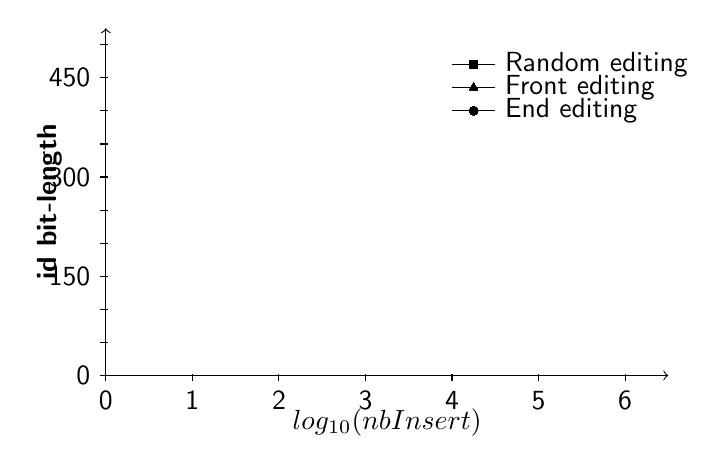
\begin{tikzpicture}[scale=0.7,x=1.57cm, y=0.6cm,font=\sffamily]

%Axis
    \draw[->] (0,0) -- coordinate (x axis mid) (6.5,0);
    \draw[->] (0,0) -- coordinate (y axis mid) (0,10.5);
%Ticks
        \foreach \x in { 0, 1, 2, 3, 4, 5, 6} { \draw (\x,1pt) -- (\x,-3pt)
          node[anchor=north] {\x};}

        \foreach \y/\ytext in { 0/0, 1/, 2/, 3/150, 4/, 5/, 6/300, 7/, 8/,
          9/450, 10/} { \draw (1pt,\y) -- (-3pt,\y) node[anchor=east] {\ytext}
          ;}
%Labels
        \node[below=0.3cm] at (x axis mid) {$log_{10}(nbInsert)$};
        \node[rotate=90, below=-1.0cm] at (y axis mid) {\textbf{id
            bit-length}};

%Plots
        \draw plot[mark=*, mark options={fill=black}] file
              {doublerandomDataQueue.data}; \draw plot[mark=triangle*, mark
                options={fill=black} ] file {doublerandomDataFront.data}; \draw
              plot[mark=square*, mark options={fill=black}] file
              {doublerandomDataRand.data};

%legend
        \begin{scope}[shift={(4,8)}]
        \draw (0,0) -- plot[mark=*, mark options={fill=black}] (0.25,0) --
        (0.5,0) node[right]{End editing}; \draw[yshift=\baselineskip] (0,0)
        -- plot[mark=triangle*, mark options={fill=black}] (0.25,0) --
        (0.5,0) node[right]{Front editing}; \draw[yshift=2*\baselineskip]
        (0,0) -- plot[mark=square*, mark options={fill=black}] (0.25,0) --
        (0.5,0) node[right]{Random editing};
        \end{scope}
\end{tikzpicture}

